\section{Introduction}
% Lukas note:
% I like to use SCQA (Situation, Complication, Question, Answer) 'system' to write the introduction, see one of the two links below
% https://analytic-storytelling.com/scqa-what-is-it-how-does-it-work-and-how-can-it-help-me/
% https://corporatefinanceinstitute.com/resources/careers/how-to-job-guides/scqa/
% https://karrierebibel.de/scqa-methode/

% 1. Describe the Current Situtation
% Functions as a starting point and a common basis. Therefore it primarily contains recognizable and agreed points.

Hardware that allows physically moving a user's body becomes increasingly lightweight and seamless. Wearable exoskeletons move a user's body by applying forces to the extremities, for example by pulling on the fingertips (see Dexmo Haptic Glove \footnote{https://www.dextarobotics.com/}) while electrical muscle stimulation (EMS) makes the user's extremities move by sending current into the muscle activating nerves.

Such technologies have primarily found application in rendering haptic sensations in virtual realities. However, with the potential to move the user's body independent of their intent, applications augmenting the user and its environment are feasible.

% 2. What is the complication, challenge identified
% Spells the reason for acting now. It contains threats / opportunities and the hurdles that need to be overcome.

if something happens for you in an interaction there is a cost to that:
- impacts sense of agency which in turn makes user's engage less
- impacts precision and accuracy, which can be very critical in high stakes scenarios, e.g. air traffic control

% 3. Question
% Asks the question how the hurdles of the Complication can be overcome. How can we prevent the threat or seize the opportunity? Also, what would be the benefits if the complication would be overcome?

But how can we build a physical augmentation system that keeps user's engaged in the action, preserving sense of agency? In other words how can we design for users to experience natural augmentation?

% 4. (short) Answer Teaser
% Provides the answer on how to overcome the hurdles. Explains how this will help deflect the threats or seize the opportunities.
% keep this short

In this paper, we present an augmentation that maintains the user's sense of agency. Our system establishes a fast communication channel between the user's thoughts and a physical end effector, here EMS. The system controls the user's muscles through EMS at the time of the user's intent to interact, as measured through readiness potentials (RP) present in the user's electroencephalogram (EEG). In our user study we then investigated whether keeping the physical impact on the user's body in line with their intention to move, preserves their sense of agency.

\subsection{Human-Computer Collaboration for Natural Augmentation: Triggering Reaching Movements at the Time of Intention}

\missingfigure{maybe small infographic here showing the connection from EEG volitional RP thoght to EMS trigger on the Arm.}

% 4. (long) Anwser with teaser image
% Provides the answer on how to overcome the hurdles. Explains how this will help deflect the threats or seize the opportunities.
% Now extend into a longer paragraph with a teaser image explaining the system in the following subsection

% for citations use use "~\cite{}" instead of " \cite{}" → no white space, copy bibtex items to cite into input/bibliography.bib
% example:


% This is what most people (90+%) will see from your paper!

% - [ ]  use hemingwayapp.com (+SEO if hardcore) to make figure captions super precise
% - [ ]  are all the axes labels readable, font size 10 or up
% - [ ]  check for missing information: give someone the figure with captions to someone neutral to check if everything is clear from the figure alone
% - [ ]  for digital version: what is alt-text of figure, i.e. when hovering with the mouse over the figure what text appears next to the cursor
% - [ ]  for accessibility: write figure caption for the blind
%     - [ ]  explain what the figure shows
%     - [ ]  refactor using hemingwayapp.com

\begin{teaserfigure}
  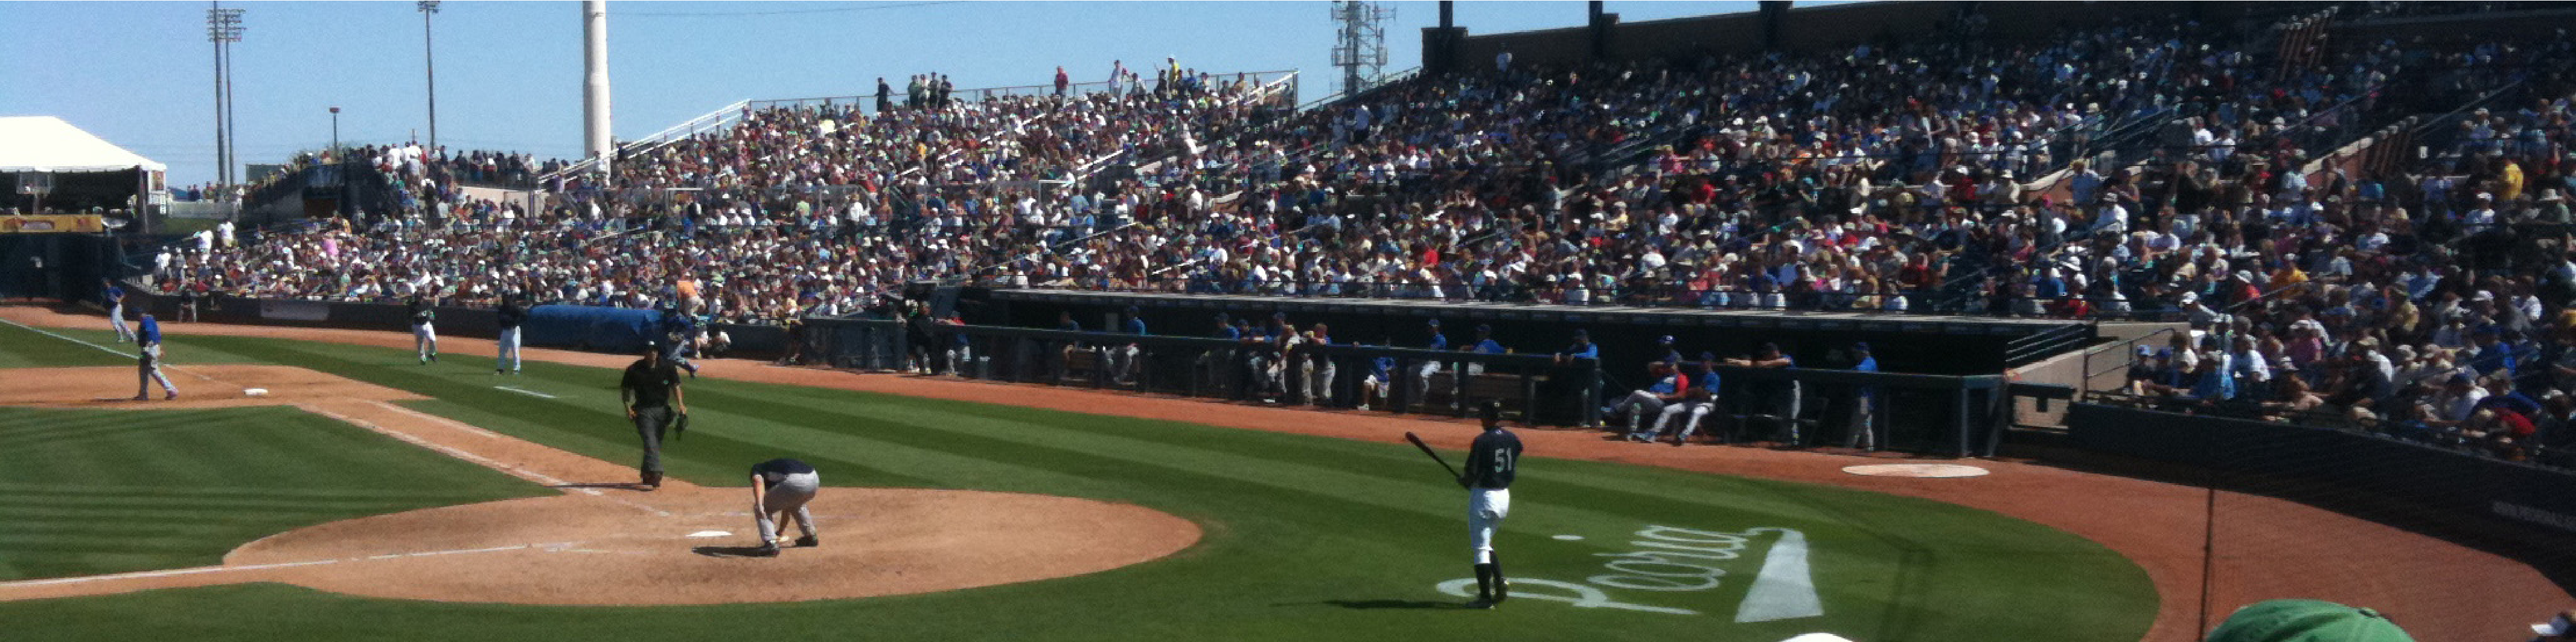
\includegraphics[width=\textwidth]{tex_sample_files/sampleteaser.pdf}
  \caption{Seattle Mariners at Spring Training, 2010.}
  \Description{Enjoying the baseball game from the third-base
  seats. Ichiro Suzuki preparing to bat.}
  \label{fig:teaser}
\end{teaserfigure}